\documentclass[border=0pt]{standalone}
\usepackage{amsmath,amssymb}
\usepackage{xcolor}
\usepackage{tikz}
\renewcommand{\sfdefault}{phv}
\usetikzlibrary{arrows.meta,fit,shapes.symbols,shapes.geometric,positioning,calc}
% --- reusable vector icons for the system-view figure ---
% figure lettering: 8 pt Helvetica, the journal's minimum (the class's \footnotesize is only 7 pt)
\newcommand{\figfont}{\sffamily\fontsize{8}{9.6}\selectfont}
\newcommand{\gnbtower}[1]{%
  \begin{scope}[shift={#1}]
    \draw[thick,gray!45!black,fill=gray!12] (-0.15,0)--(0,0.82)--(0.15,0)--cycle;
    \draw[gray!55!black] (-0.095,0.28)--(0.095,0.28) (-0.065,0.46)--(0.065,0.46) (-0.035,0.63)--(0.035,0.63);
    \fill[gray!55] (-0.12,0.64) rectangle (-0.03,0.84);
    \fill[gray!55] (0.03,0.64) rectangle (0.12,0.84);
    \draw[blue!55!black] (0.17,0.72) arc (-55:55:0.13);
    \draw[blue!55!black] (0.22,0.68) arc (-55:55:0.21);
    \draw[blue!55!black] (-0.17,0.72) arc (235:125:0.13);
    \draw[blue!55!black] (-0.22,0.68) arc (235:125:0.21);
  \end{scope}
}
\newcommand{\uephone}[2]{%
  \begin{scope}[shift={#1}]
    \draw[thick,#2!65!black,fill=#2!14,rounded corners=1pt] (-0.12,-0.2) rectangle (0.12,0.2);
    \fill[#2!30] (-0.08,-0.09) rectangle (0.08,0.13);
    \fill[#2!65!black] (0,-0.15) circle (0.016);
  \end{scope}
}

\begin{document}
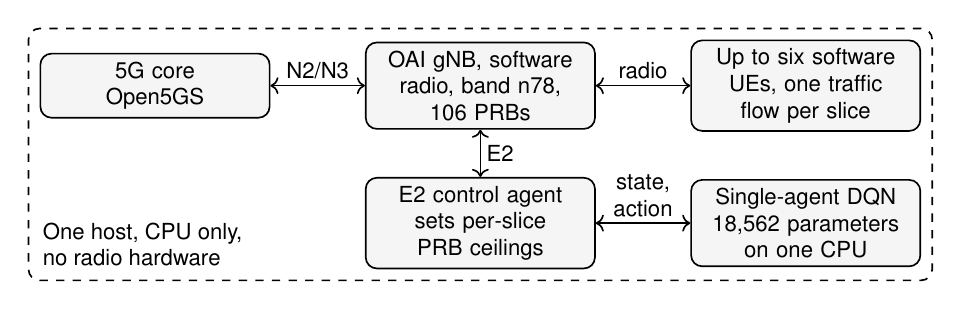
\begin{tikzpicture}[
  blk/.style={draw, semithick, rounded corners, align=center, fill=gray!8, font=\figfont, inner sep=3pt, text width=2.7cm},
  arr/.style={-{Latex[length=2mm]}, semithick},
  lbl/.style={font=\figfont, inner sep=1pt}
]
\node[blk] (core) at (0,0) {5G core\\ Open5GS};
\node[blk, right=1.2cm of core] (ran) {OAI gNB, software\\ radio, band n78,\\ 106 PRBs};
\node[blk, right=1.2cm of ran] (ues) {Up to six software\\ UEs, one traffic\\ flow per slice};
\node[blk, below=0.6cm of ran] (ctrl) {E2 control agent\\ sets per-slice\\ PRB ceilings};
\node[blk] (pol) at (ues |- ctrl) {Single-agent DQN\\ 18{,}562 parameters\\ on one CPU};
\draw[arr, <->] (core) -- (ran) node[lbl, midway, above=1pt] {N2/N3};
\draw[arr, <->] (ran) -- (ues) node[lbl, midway, above=1pt] {radio};
\draw[arr, <->] (ran) -- (ctrl) node[lbl, midway, right=1pt] {E2};
\draw[arr, <->] (ctrl) -- (pol) node[lbl, midway, above=1pt, align=center] {state,\\ action};
\node[draw, semithick, dashed, rounded corners, inner sep=4pt, fit=(core)(ran)(ues)(ctrl)(pol)] (host) {};
\node[font=\figfont, align=left, anchor=south west, inner sep=1pt] at ([xshift=0.15cm]host.west |- ctrl.south) {One host, CPU only,\\ no radio hardware};
\end{tikzpicture}
\end{document}
